\chapter{Conclusions}

\section{Does flu evolve like we think it does?}

In \citet{Barrat-Charlaix2020}, we investigated the predictability of flu mutation frequencies.
We explicitly avoided modeling flu evolution and focused on an empirical account of long-term outcomes for mutation frequency trajectories.
We selected all available HA and NA sequences for flu lineages A/H3N2 and A/H1N1pdm, performed multiple sequence alignments per lineage and gene, binned sequences by month, and calculated the frequencies of mutations per site and month.
From these data, we constructed frequency trajectories of individual mutations that were rising in frequency from zero.
We expected these rising mutations to represent beneficial, large-effect mutations that would sweep through the global population as predicted by the population genetic theory described above.
By considering individual mutations, we effectively averaged the outcomes of these mutations across all genetic backgrounds.
We evaluated the outcomes of trajectories for mutations that had risen from 0\% to approximately 30\% global frequency and classified trajectories for mutations that fixed, died out, or persisted as polymorphisms.

\begin{figure}
  \centering
  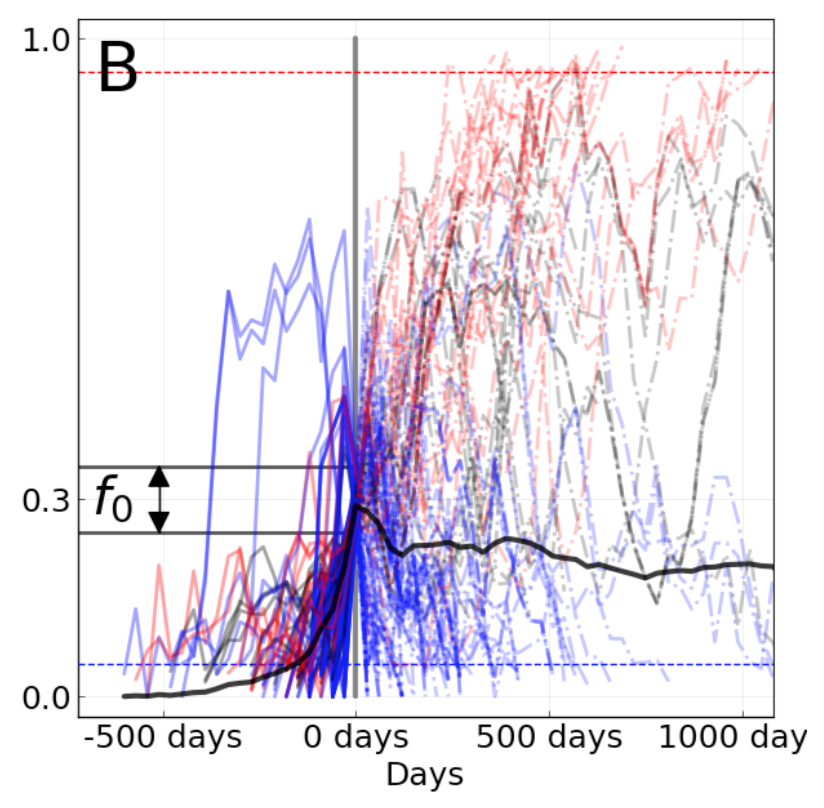
\includegraphics[width=0.75\textwidth]{chapter_05/flu-forecasting-mutation-trajectories-static.png}
  \caption[{Mutation trajectories for seasonal influenza A/H3N2 where mutations rose from a frequency of zero to approximately 30\% frequency.}]{{\bf Mutation trajectories for seasonal influenza A/H3N2 where mutations rose from a frequency of zero to approximately 30\% frequency.}
    Dashed horizontal lines represent thresholds for fixation (red) and loss (blue).
    Trajectory colors also indicate eventual fixation (red), loss (blue), or persistence as a polymorphism (black).
    The thick black dashed line indicates the average frequency of all trajectories shown.
    For the interactive figure, hover over individual trajectories to highlight their full extent and details about the current frequency of a given mutation at each timepoint.
    Use the radio buttons to filter trajectories by segment and outcome.
    (After Figure 1B in \citet{Barrat-Charlaix2020}.)
    \href{https://bedford.io/blog/predicting-seasonal-influenza-evolution/\#mutation-trajectories}{Explore an interactive version of this figure}.\label{fig:mutation-trajectories} }
\end{figure}

The average trajectory of individual rising A/H3N2 mutations failed to rise toward fixation (Figure~\ref{fig:mutation-trajectories}).
Instead, the future frequency of these mutations was no higher on average than their initial frequency.
We repeated this analysis for mutations with initial frequencies of 50\% and 75\% and for mutations in A/H1N1pdm and found nearly the same results.
From these results, we concluded that it is not possible to predict the short-term dynamics of individual mutations based solely on their recent success.

Next, we calculated the fixation probability of each mutation trajectory based on its initial frequency.
Surprisingly, we found that the fixation probabilities of A/H3N2 mutations were equal to their initial frequencies.
This pattern corresponds to what we expect for mutations evolving neutrally, where population genetic theory predicts that fixation probability is equal to current mutation frequency.
Generally, the pattern remained the same even when we binned mutations by high LBI, presence at epitope sites, multiple appearances of a mutation in a tree, geographic spread, or other potential metrics associated with high fitness.
We concluded that the recent success of rising mutations provides no information about their eventual fixation.

We tested whether we could explain these results by genetic linkage or clonal interference by simulating flu-like populations under these evolutionary constraints.
Mutation trajectories from simulated populations were more predictable than those from natural populations.
The closest our simulations came to matching the uncertainty of natural populations was when we dramatically increased the rate at which the fitness landscape of simulated populations changed.
These results suggested that we cannot explain the unpredictable nature of flu mutation trajectories by linkage or clonal interference alone.

Since flu mutation trajectories lacked ``momentum'' and LBI did not provide information about eventual fixation of mutations, we wondered whether we could identify the most representative sequence of future populations with a different metric.
The consensus sequence is provably the best predictor for a neutrally evolving population.
We found that the consensus sequence is often closer to the future population than the virus sequence with the highest LBI.
Indeed, we found that the top LBI virus was frequently similar to the consensus sequence and often identical.

Taken together, our results from this empirical analysis reveal that beneficial mutations of large effect do not predictably sweep through flu populations and fix.
Instead, the average outcome for any individual mutation resembles neutral evolution, despite the strong positive selection expected to act on these mutations.
Although simulations rule out clonal interference between large effect mutations as an explanation for these results, we cannot discount the role of multiple mutations of similar, smaller effects in the overall fitness of flu viruses and the fixation of multiple co-evolving mutations.

\section{Can we forecast flu evolution?}

In \citet{Huddleston2020}, we built a modeling framework based on the approach described in \citet{Luksza:2014hj} to forecast flu A/H3N2 populations one year in advance.
We used this framework to predict the sequence composition of the future population, the frequency dynamics of clades, and the virus in the current population that most represented the future population.
As in \citet{Barrat-Charlaix2020} and \citet{Luksza:2014hj}, we assumed that viruses grow exponentially as a function of their fitness and that viruses with similarly high fitness compete with each other under clonal interference.
In contrast to \citet{Barrat-Charlaix2020}, we considered the fitness of complete amino acid haplotypes instead of individual mutations.

We estimated fitness with metrics based on HA sequences and experimental measurements of antigenic drift and functional constraint.
The sequence-based metrics included the epitope cross-immunity and mutational load estimates defined by \citet{Luksza:2014hj}, LBI from \citet{Neher:2014eu}, and ``delta frequency'', a measure of recent change in clade frequency analogous to Barrat-Charlaix's rising mutations.
The experimental metrics included a cross-immunity measure based on hemagglutination inhibition (HI) assays \citep{Neher:2016hy} and an estimate of functional constraint based on mutational preferences from deep mutational scanning experiments \citep{Lee2018}.

We trained models based on each of these metrics independently and in relevant combinations of complementary metrics.
For each model, we fit coefficients per fitness metric that minimized the distance between the estimated and observed amino acid haplotype composition of the future (Figure~\ref{fig:model}).
These coefficients represent the effect of each metric on flu fitness.
As a control, we also calculated the distance to the future population for a ``naive'' model that assumed the future population is the same as the current population.
To test our framework, we simulated 40 years of evolution for flu-like populations with SANTA-SIM and fit models to these data.
After verifying our framework with simulated populations, we trained models for natural A/H3N2 populations using 25 years of historical data.
We tested the accuracy of each model by applying the coefficients from the training data to forecasts of new out-of-sample data from the last 5 years of A/H3N2 evolution.

\begin{figure}
  \begin{center}
  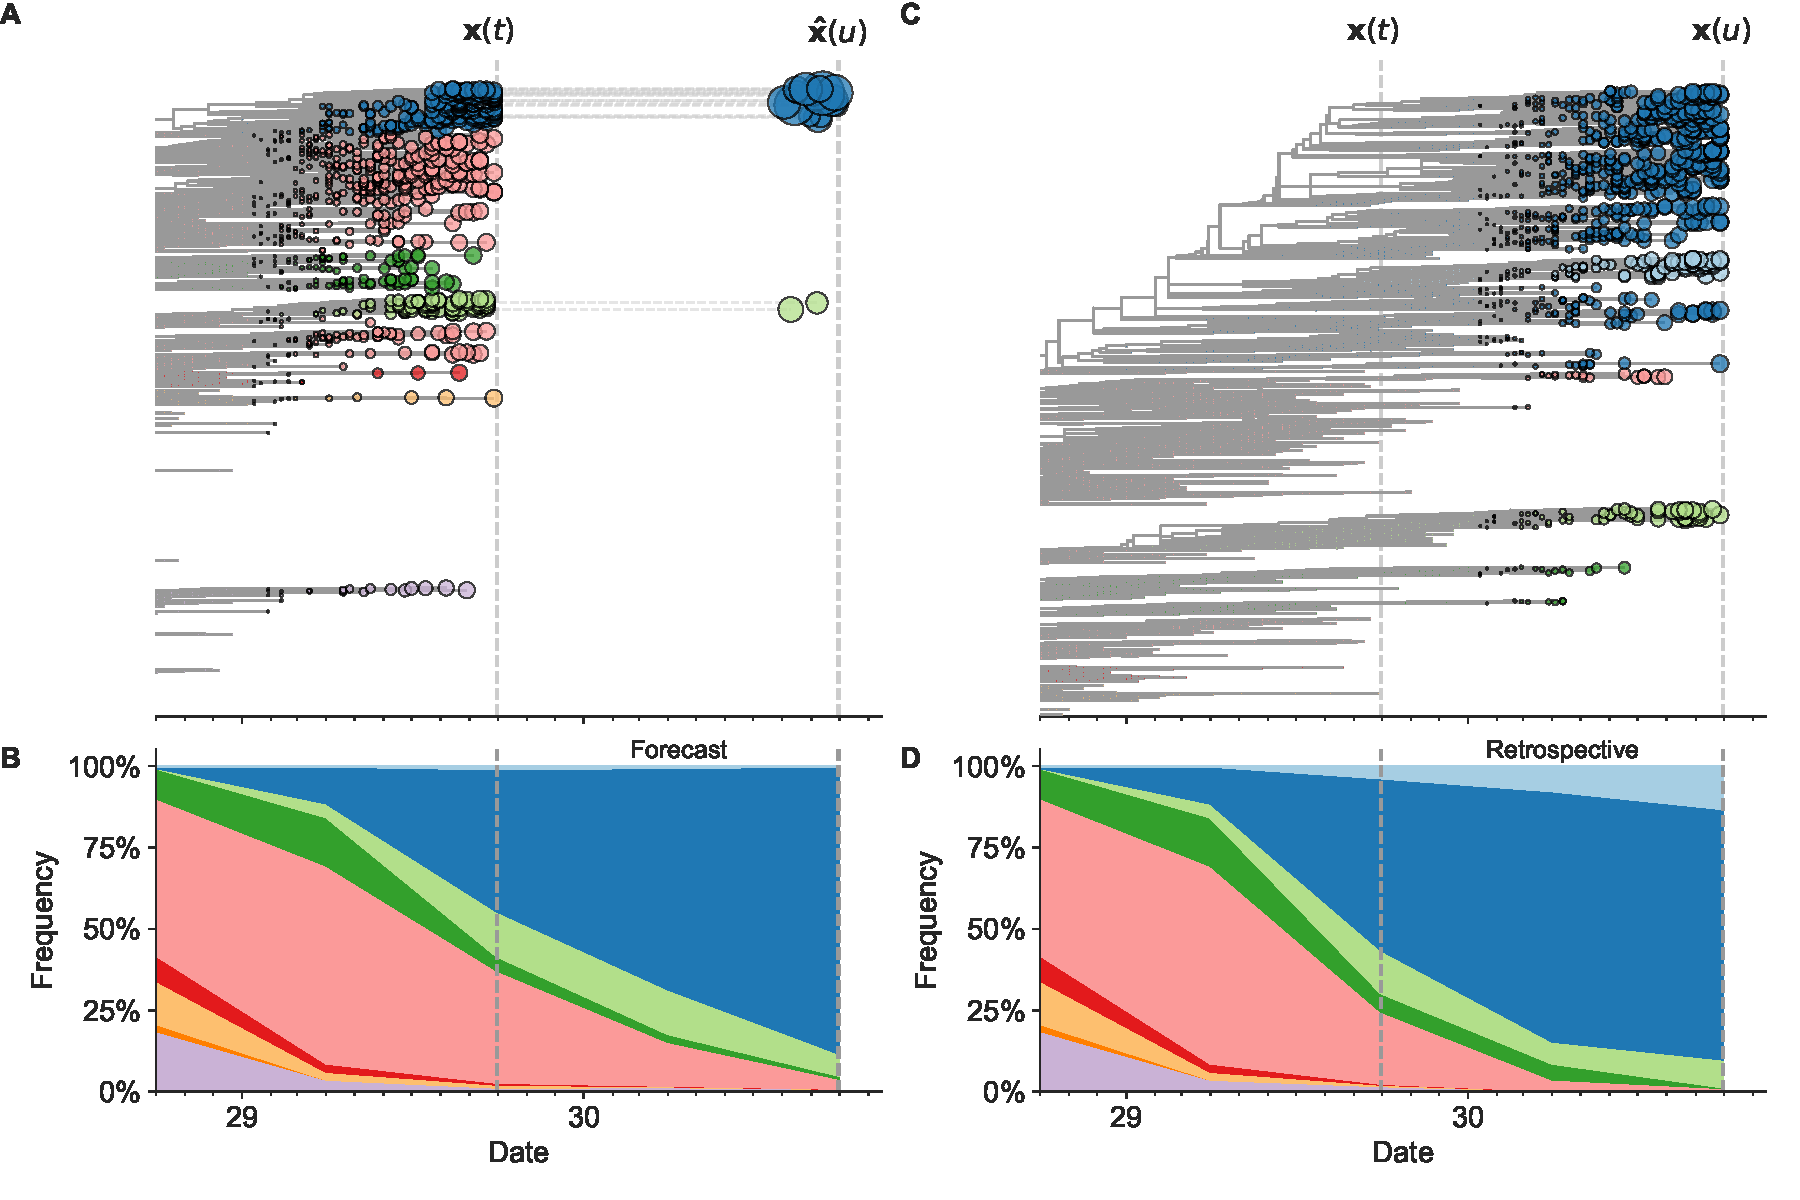
\includegraphics[width=\columnwidth]{chapter_04/Figure_1.pdf}
  \caption[{Schematic representation of the fitness model for simulated H3N2-like populations.}]{
    {\bf Schematic representation of the fitness model for simulated H3N2-like populations.}
    The fitness of strains at timepoint $t$ determines the estimated frequency of strains with similar sequences one year in the future at timepoint $u$.
    Genetically similar strains by amino acid sequence have similar colors.
    A) Strains at timepoint $t$, $\mathbf{x}(t)$, are shown in their phylogenetic context and sized by their frequency at that timepoint.
    The estimated future population at timepoint $u$, $\mathbf{\hat{x}}(u)$, is projected to the right with strains scaled in size by their projected frequency based on the known fitness of each simulated strain.
    B) The frequency trajectories of strains at timepoint $t$ to $u$ represent the predicted the growth of the dark blue strains to the detriment of the pink strains.
    C) Strains at timepoint $u$, $\mathbf{x}(u)$, are shown as in panel A.
    D) The observed frequency trajectories of strains at timepoint $u$ broadly recapitulate the model's forecasts while also revealing increased diversity of sequences at the future timepoint that the model could not anticipate.
  }
  \label{fig:model}
  \end{center}
\end{figure}

We found that the most robust forecasts depended on a combined model of experimentally-informed antigenic drift and sequence-based mutational load.
Importantly, this model explicitly accounts for the benefits of antigenic drift and the costs of deleterious mutations.
This model also slightly outperformed the naive model in its estimation of future clade frequencies.
However, we found that the naive model often selected individual strains that were as close to the future population as the best biologically-informed model.
The naive model's estimated closest strain to the future is effectively the weighted average of the current population and conceptually similar to the consensus sequence of the population.
From these results, we concluded that the predictive gains of fitness models depend on the prediction target.

Surprisingly, the sequence-based metrics of epitope cross-immunity and delta frequency and the mutational preferences from DMS experiments had little predictive power.
These metrics failed to make accurate forecasts because of their dependence on a specific historical context.
For example, the original epitope cross-immunity metric \citep{Luksza:2014hj} depends on a predefined list of epitope sites that were originally identified in a retrospective study of flu sequences up through 2005 \citep{Shih:2007bd}.
This metric correspondingly failed to predict the future after 2005, suggesting that its previous success depended on inadvertently borrowing information from the future.
Similarly, the mutational preferences from DMS experiments measure effects of all single amino acid mutations to the genetic background of the virus A/Perth/16/2009.
The metric based on these preferences failed to predict the future after 2009, reflecting the strong dependence of these preferences on their original genetic background.
Both delta frequency and LBI suffered from overfitting to the training data, in a more general form of historical dependence.

\section{How do results from our two studies compare?}

The two studies we have presented here use different approaches to analyze the same natural flu populations.
We completed these two studies mostly independently and have only now begun to reconcile their findings.
We were especially interested to understand how simulated populations from the two studies differed and whether the optimal predictor from \citet{Barrat-Charlaix2020} could also be an accurate fitness metric in the modeling framework from \citet{Huddleston2020}.

Simulated populations play an important role in our two studies.
We generated these simulated data as a source of truth where we understand the population dynamics because we defined them.
In \citet{Barrat-Charlaix2020}, the simulated binary populations from ffpopsim \citep{Zanini2012} evolved under strong epistasis and immune escape pressure.
These populations showed us that mutation trajectories could be predictable under these population genetic constraints.
In \citet{Huddleston2020}, the simulated nucleotide populations from SANTA-SIM \citep{Jariani2019} also evolved under strong epistasis, purifying selection, and an ``exposure dependent'' fitness function that mimics immune escape pressure.
We used these populations to confirm that our forecasting framework could accurately predict the composition of future populations.
Interestingly, when we inspected the predictability of the mutation trajectories for these simulated populations, we found that they resembled the weak predictability of natural H1N1pdm trajectories (Figure~\ref{fig:mutation-trajectories-comparison}).
Despite the weak predictability of mutation trajectories from these simulated populations, we were able to forecast the composition of their future populations.
These results highlight the importance of using complete haplotypes to make predictions, as individual mutation trajectories remain difficult to predict.

\begin{figure}
  \begin{subfigure}[b]{0.5\textwidth}
    \centering
    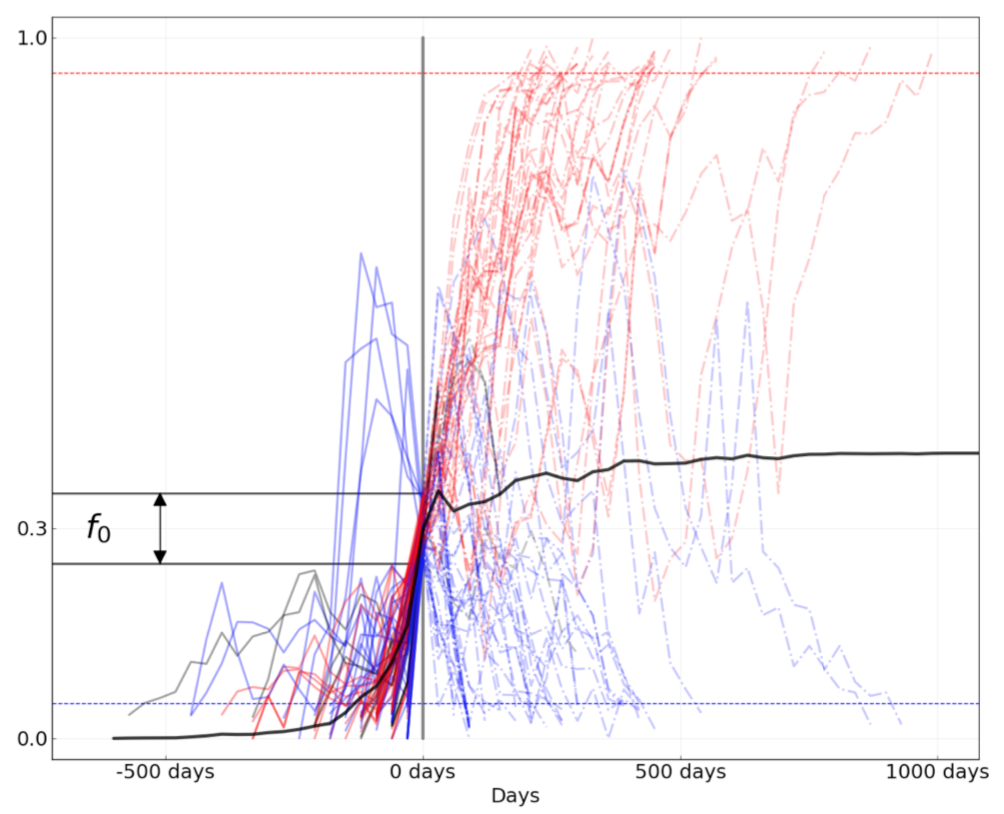
\includegraphics[width=\textwidth]{chapter_05/flu-forecasting-mutation-trajectories-h1n1pdm.png}
    \label{fig:mutation-trajectories-h1n1pdm}
  \end{subfigure}
  \hfill
  \begin{subfigure}[b]{0.4\textwidth}
    \centering
    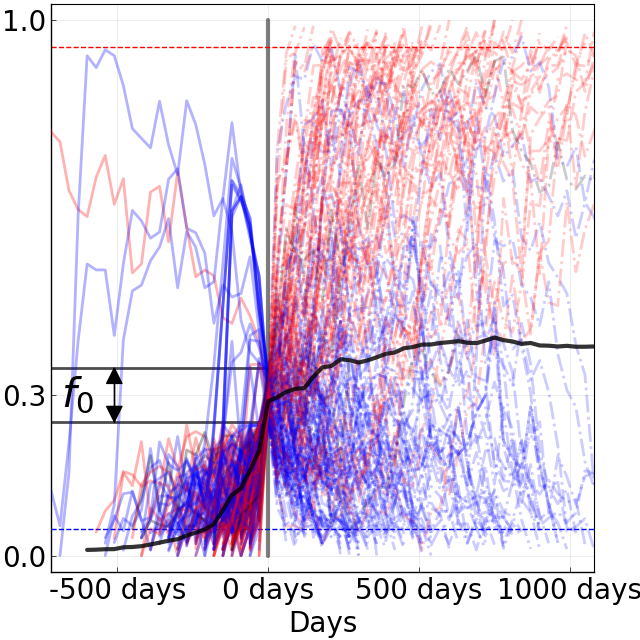
\includegraphics[width=\textwidth]{chapter_05/flu-forecasting-rising_trajectories_f03.png}
    \label{fig:mutation-trajectories-simulated}
  \end{subfigure}

  \caption[{Comparison of rising trajectories for natural H1N1pdm trajectories from \citet{Barrat-Charlaix2020} and simulated flu-like populations from \citet{Huddleston2020}.}]{{\bf Comparison of rising trajectories for natural H1N1pdm trajectories from \citet{Barrat-Charlaix2020} and simulated flu-like populations from \citet{Huddleston2020}.}
    A) Rising trajectories for H1N1pdm mutations as reported in Figure S9 of \citet{Barrat-Charlaix2020}.
    B) Rising trajectories for flu-like populations simulated with SANTA-SIM in \citet{Huddleston2020}.
    Mutation trajectories from simulated populations resemble those of natural H1N1pdm mutations.\label{fig:mutation-trajectories-comparison}
  }
\end{figure}

We also wanted to know whether the optimal metric from \citet{Barrat-Charlaix2020} for selecting a representative of the future, the consensus sequence of the current population, could make accurate forecasts in the modeling framework from \citet{Huddleston2020}.
We noted above that the closest strain to the future selected by the naive model from \citet{Huddleston2020} is analogous to the consensus sequence of the current population.
One important difference is that the naive model has to select a previously sampled strain while the consensus sequence represents a hypothetical strain that may not exist in nature.
To understand whether the consensus sequence could also improve forecasts of the future population's haplotype composition, we developed a new fitness metric called the ``distance from consensus''.
For each timepoint in our forecasting analysis, we constructed the amino acid consensus sequence from all extant strains and calculated the pairwise distance between the consensus and each extant strain.
If the consensus sequence is the best representation of the future population, we expected the corresponding model's coefficients to be consistently negative.
This negative coefficient would have the effect of penalizing strains whose amino acid sequences diverged greatly from the consensus sequence.

\begin{figure}
  \centering
  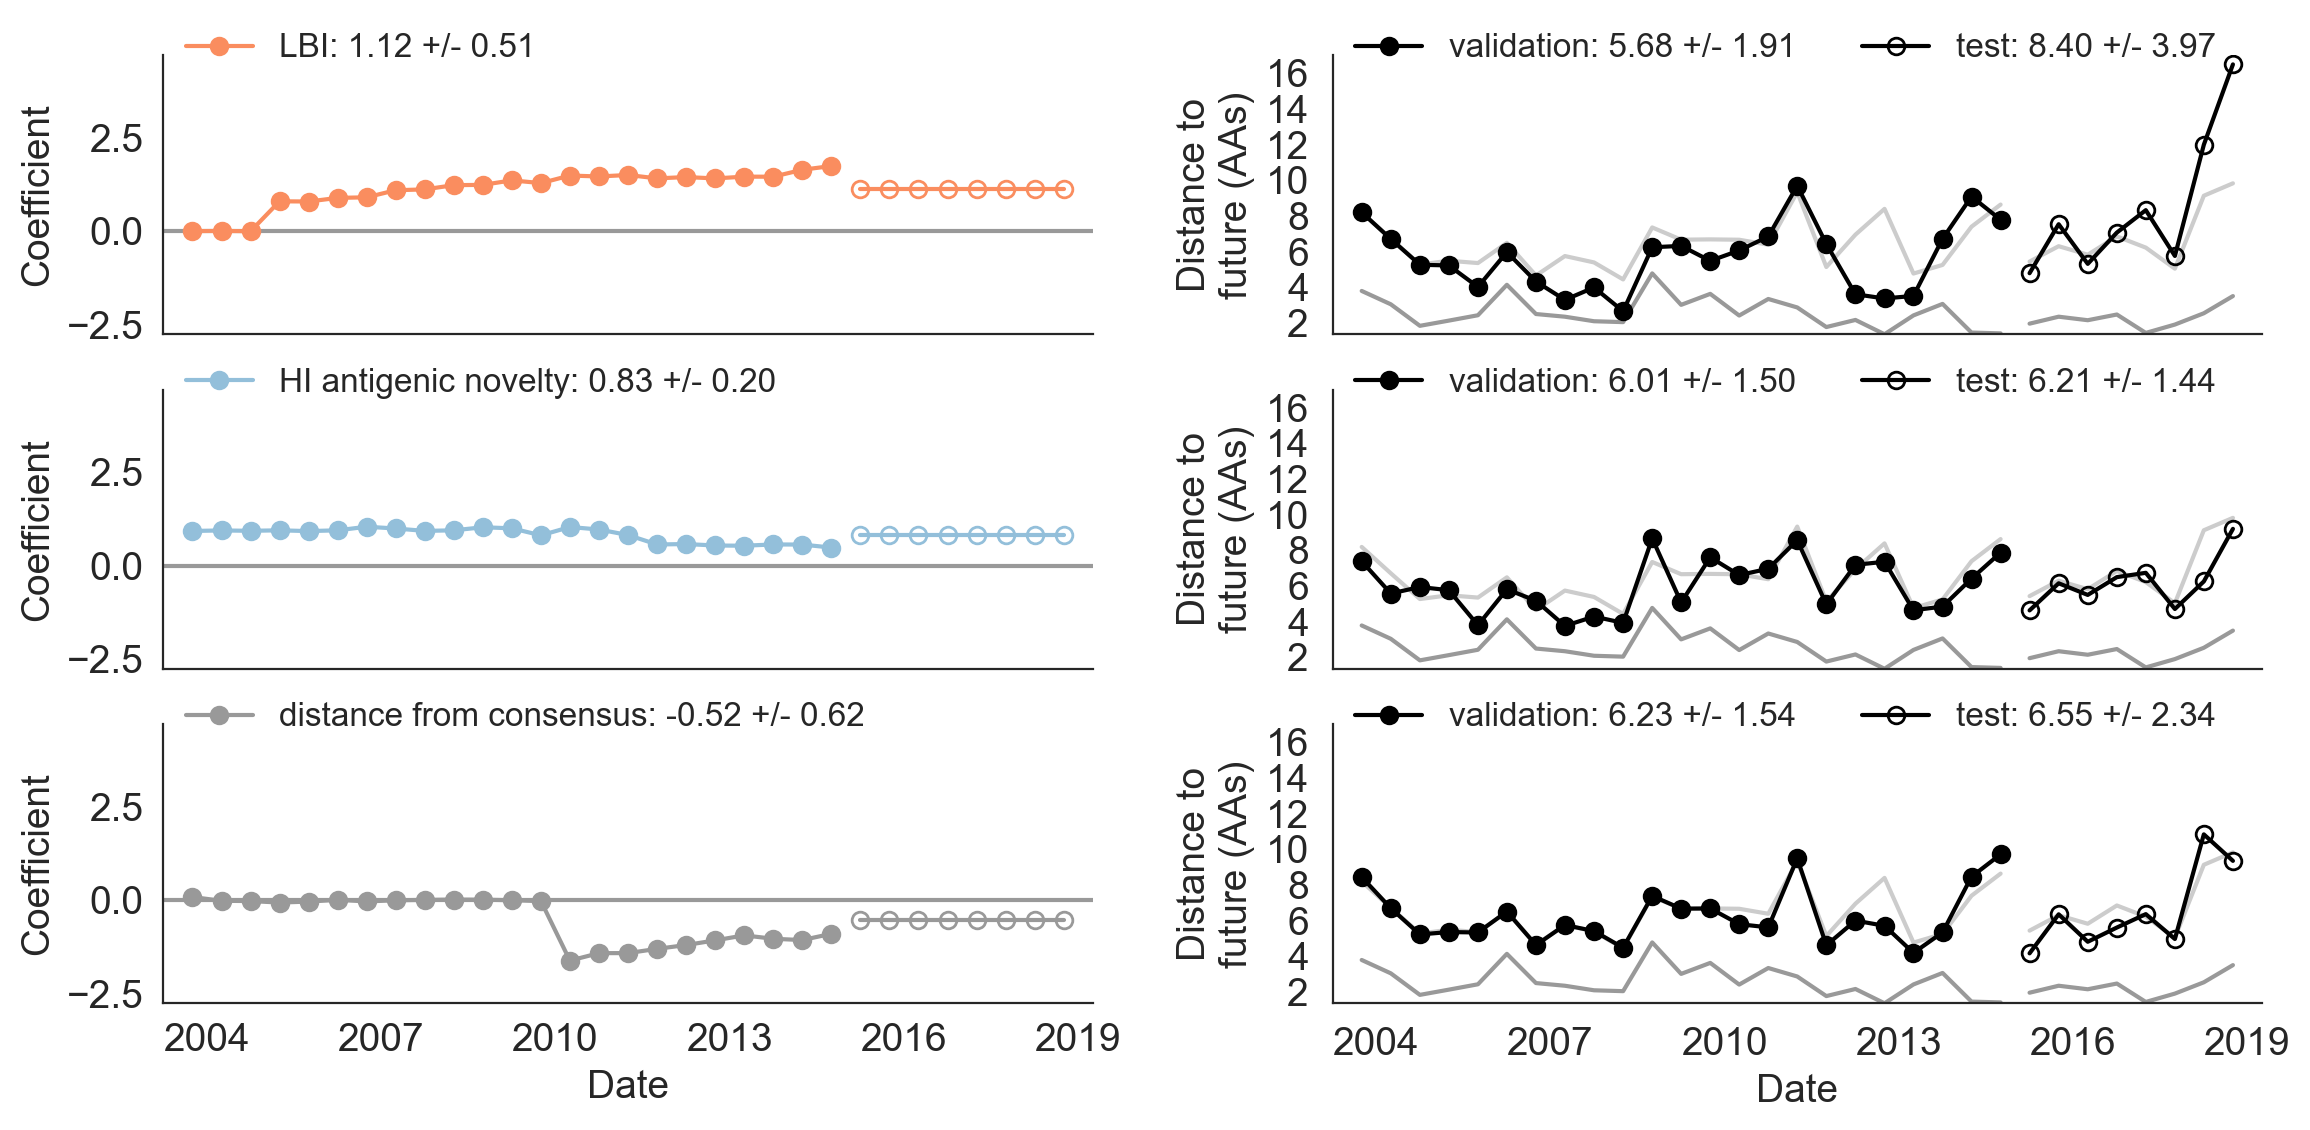
\includegraphics[width=\textwidth]{chapter_05/flu-forecasting-distance-to-consensus-vs-lbi-and-hi.png}
  \caption[{Model coefficients and distance to the future for LBI, HI antigenic novelty, and distance from consensus metrics.}]{{\bf Model coefficients and distance to the future for LBI, HI antigenic novelty, and distance from consensus metrics.}
    A) Coefficients are shown per validation timepoint (solid circles, N=23) with the mean +/- standard deviation in the top-left corner.
    For model testing, coefficients were fixed to their mean values from training/validation and applied to out-of-sample test data (open circles, N=8).
    B) Distances between projected and observed populations are shown per validation timepoint (solid black circles) or test timepoint (open black circles).
    The mean +/- standard deviation of distances per validation timepoint are shown in the top-left of each panel.
    Corresponding values per test timepoint are in the top-right.
    The naive model's distance to the future (light gray) was 6.40 +/- 1.36 AAs for validation timepoints and 6.82 +/- 1.74 AAs for test timepoints.
    The corresponding lower bounds on the estimated distance to the future (dark gray) were 2.60 +/- 0.89 AAs and 2.28 +/- 0.61 AAs.\label{fig:distance-to-consensus-performance} }
\end{figure}

We fit a model to this new metric using the same 25 years of historical A/H3N2 data described in \citet{Huddleston2020} and tested the robustness of the model on the last 5 years of A/H3N2 data.
We compared the performance of this model to models for LBI and experimental measures of antigenic drift (HI antigenic novelty).
For the first half of the training period, the distance to consensus metric received a coefficient of zero, meaning it did not improve forecasts over the naive model (Figure~\ref{fig:distance-to-consensus-performance}).
In the second half of the training period, the metric received a strong negative coefficient, as we expected.
When we applied the mean coefficient from the training period to out-of-sample data in the test period, we found that the distance from consensus metric outperformed LBI and performed only slightly worse than the antigenic drift metric.
These results support findings from both of our studies.
The consensus sequence is a more robust representative of the future than LBI, as shown in \citet{Barrat-Charlaix2020}.
However, experimental measurements of antigenic drift still provide more information about the future population than sequence-only metrics, as shown in \citet{Huddleston2020}.
We anticipate that this new distance from consensus metric could eventually replace the existing mutational load metric in a combined model with HI antigenic novelty.
This new combined model could potentially provide better estimates of functional constraint (by limiting changes from the consensus) and antigenic drift (by using experimental measures of antigenic drift phenotypes.)

\section{How have these results changed how we think about flu evolution?}

In general, we found that the evolution of H3N2 flu populations remains difficult to predict.
The frequency dynamics and fixation probabilities of individual mutations resemble neutrally evolving alleles.
We can weakly predict the frequency dynamics of flu clades when we combine experimental and genetic data in models that account for antigenic drift and mutational load.
In the best case, we can use these same biologically-informed models to predict the sequence composition of future flu populations.
However, these complex fitness models do not always outperform simpler models, when predicting which individual virus is the most representative of the future population.
In \citet{Barrat-Charlaix2020}, the consensus sequence of the current population was as close or closer to the future population than the sequence with the highest local branching index.
In \citet{Huddleston2020}, a naive model estimated the single closest strain to the future nearly as well as the best biologically-informed models.

Successful flu predictions depend on the choice of prediction targets and fitness metrics.
Future prediction efforts should attempt to estimate the composition of future populations instead of future clade frequencies.
Fitness models should account for the genetic background of beneficial mutations and favor fitness metrics that are the least susceptible to model overfitting and historical contingency.
The benefits of considering the genetic background of individual mutations in HA suggest that considering the context of all genes should yield gains, too.
We need measures of antigenic drift from human antisera to complement current measures based on ferret antisera.
We may also improve forecast accuracy by accounting for flu's global migration patterns.
Most importantly, we should make the forecasting problem itself easier by embracing efforts to reduce the lag between vaccine composition decisions and distribution to the public.

With a validated forecasting framework in hand, we can readily produce real-time forecasts at nextstrain.org and as part of recommendations submitted to the World Health Organization prior to biannual vaccine composition meetings \cite{Bedford780627}.
Other modeling groups produce similar reports with forecasts of even higher precision.
However, there is no expectation or formal requirement for us to revisit and evaluate the accuracy of our predictions.
The long-term historical accuracy of forecasting models does not matter, if these models fail to perform consistently in modern forecasts.
For this reason, we recommend that modeling groups formally archive their forecasts for each composition meeting and periodically assess the performance of their models in real forecasting conditions.
Modeling groups that participate in short-term or within-season flu forecasts have already adopted this approach, as part of the CDC Flusight network.
The Zoltar Forecast Archive \citep{reich2020zoltar} was designed with these forecasts in mind and could be modified to support storage of long-term forecasts.
We expect that these formal archives of real forecasts will improve accountability of modeling groups, increase the accuracy of forecasts made by their models, and encourage community consensus on model targets.
